% !TeX root = er.tex

\chapter{Aprendizagem da máquina}\label{ch.machine}

Considere um robô que reconhece e agarra objetos amarelos (Fig.~\ref{fig.sortballs}). Ele pode usar uma câmera colorida para identificar objetos amarelos, mas os objetos aparecerão diferentes em ambientes diferentes, como na luz do sol, em uma sala escura ou em um showroom. Além disso, é difícil definir com precisão o que significa "amarelo": qual é o limite entre amarelo e amarelo limão-amarelo ou entre amarelo e laranja? Em vez de escrever instruções detalhadas para o robô, preferimos que o robô aprenda a reconhecer as cores enquanto executa a tarefa, para que ele possa se adaptar ao ambiente onde a tarefa acontece. Especificamente, queremos projetar um algoritmo de \emph{classificação} que possa ser \emph{treinado} para executar a tarefa sem fornecer todos os detalhes com antecedência.

\begin{figure}
\begin{center}
\includegraphics[width=0.8\textwidth]{sorting-robot.jpg}
\end{center}
\caption{Bolas coloridas para classificação de braços robóticos}\label{fig.sortballs}
\end{figure}

Os algoritmos de classificação são um tópico central em \emph{machine learning}, um campo da ciência da computação e estatística que desenvolve computações para reconhecer padrões e prever resultados sem programação explícita. Estes algoritmos extraem \emph{rules} dos dados brutos adquiridos pelo sistema durante um período de treinamento. As regras são posteriormente utilizadas para classificar um novo objeto e, em seguida, para tomar a ação apropriada de acordo com a classe do objeto. Para a tarefa de reconhecimento de cores, treinamos o robô apresentando objetos de cores diferentes e dizendo ao robô quais objetos são amarelos e quais não são. O algoritmo de aprendizagem da máquina gera uma regra para a classificação de cores. Quando é apresentado com novos objetos, ele usa a regra para decidir quais objetos são amarelos e quais não são.

O capítulo anterior apresentou redes neurais artificiais que realizam uma forma de aprendizagem da máquina baseada em \emph{reinforcement}. Neste capítulo, discutimos técnicas estatísticas baseadas em \emph{supervised learning}: durante o período de treinamento, dizemos ao robô as respostas precisas, tais como se um objeto é amarelo ou não. A seção~\ref{s.sorting-onesensor} introduz as técnicas estatísticas desenvolvendo um algoritmo para distinguir entre objetos de duas cores. Apresentamos uma técnica para aprendizagem da máquina chamada \emph{linear discriminant analysis (LDA)}. As seções~~\ref{s.lda}--\ref{s.gen-lda} apresentam a LDA no mesmo contexto de distinção entre duas cores. A LDA é baseada na suposição de que os dados têm propriedades estatísticas específicas; se estas não se mantiverem, \emph{perceptrons} pode ser usada para classificação, como descrito na seção Sect.~\ref{s.perceptrons}.

Este capítulo assume que você está familiarizado com os conceitos de \emph{mean}, \emph{variance} e \emph{covariance}. Tutoriais sobre estes conceitos aparecem em Apêndices~\ref{a.mean}--\ref{a.covariance}.

\section{Distinguindo entre duas cores}\label{s.sorting-onesensor}

Começamos com o problema de distinguir as bolas amarelas das não amarelas. Para simplificar a tarefa, modificamos o problema para um de distinguir as áreas cinza escuro das áreas cinza claro que são impressas em papel colado ao chão (Fig.~\ref{fig.closegrays1}). O robô usa dois sensores terrestres que recolhem amostras da luz refletida à medida que o robô se move sobre as duas áreas.

\begin{figure}
\begin{center}
\begin{tikzpicture}[scale=.8]
\pic at (-2.2,1) { robot };
\draw[fill,gray] (-1,.6) rectangle +(6pt,8pt);
\draw[fill,gray] (-1,1.2) rectangle +(6pt,8pt);
\draw[fill,color=black!60]  (0,0) rectangle +(3.5,2);
\draw[fill,color=black!20] (4,0) rectangle +(3.5,2);
\end{tikzpicture}
\end{center}
\caption{Distinguindo duas tonalidades de cinza}\label{fig.closegrays1}
\end{figure}

A figura~\ref{fig.closegrays2} mostra um gráfico dos valores retornados pela amostragem dos dois sensores.\footnote{Os dados utilizados neste capítulo são dados reais extraídos de uma experiência com o robô Thymio.} O robô leva cerca de $70$ segundos para mover-se da esquerda para a direita, colhendo a luz refletida uma vez por segundo. É fácil ver que os dados mostram uma variação significativa, que provavelmente se deve ao ruído nos sensores e à impressão irregular. Ainda mais problemática é a variabilidade nos resultados retornados pelos dois sensores. Como o robô pode aprender a distinguir entre as tonalidades de cinza dada a variabilidade nas amostras e nos sensores? Queremos criar automaticamente uma regra para distinguir entre as duas tonalidades de cinza.

\begin{figure}
\begin{center}
\includegraphics[width=0.8\textwidth]{gray-fig.pdf}
\end{center}
\caption{Lotes de luz refletida vs. tempo para o sensor esquerdo (superior) e o sensor direito (inferior)}\label{fig.closegrays2}
\end{figure}

\subsection{Um discriminante com base nos meios}

Ao examinar as parcelas na Fig.~\ref{fig.closegrays2}, é fácil ver quais amostras são da área cinza escuro e quais são da área cinza claro. Para o sensor esquerdo, os valores da área cinza claro estão na faixa de $500$--$550$, enquanto os valores da área cinza escuro estão na faixa de $410$--$460$. Para o sensor direito, os valores estão na faixa de $460$--$480$ e $380$--$400$. Para o sensor esquerdo, um limiar de $480$ distinguiria claramente entre cinza claro e cinza escuro, enquanto para o sensor direito, um limiar de $440$ distinguiria claramente entre cinza claro e cinza escuro. Mas como estes valores ótimos podem ser escolhidos automaticamente e como podemos reconciliar os limites dos dois sensores?

Vamos primeiro nos concentrar no sensor esquerdo. Estamos procurando um \emph{discriminante}, um valor que distinga as amostras das duas cores. Considere os valores $\mathit{max}_\sub{dark}$, o valor máximo retornado pela amostragem cinza escuro, e $\mathit{min}_\sub{light}$, o valor mínimo retornado pela amostragem cinza claro. Sob a suposição razoável de que  $\mathit{max}_\sub{dark} <\mathit{min}_\sub{light}$, qualquer valor $x$ tal que $\mathit{max}_\sub{dark} < x <\mathit{min}_\sub{light}$ consegue distinguir entre os dois tons de cinza. O ponto médio entre os dois valores parece oferecer o discriminante mais robusto.

Da Fig.~\ref{fig.closegrays2} vemos que $\mathit{max}_\sub{dark}\approx 460$ ocorre a cerca de $10$ s e $\mathit{min}_{\sub{light}}\approx 500$ ocorre a cerca de $60$ s, por isso escolhemos sua média de $480$ como o discriminante. Embora isto seja correto para este conjunto de dados em particular, em geral não é uma boa idéia usar os valores máximos e mínimos porque eles poderiam ser {outliers}: valores extremos resultantes de circunstâncias incomuns, tais como um buraco no papel que retornaria incorretamente um valor muito alto na área cinza escura.

Uma solução melhor é usar \emph{all} os dados e a função mais simples de todos os dados é o \emph{mean} dos valores. Deixe que $\mu_{\sub{dark}}$ denotem a média das amostras cinzas escuras e $\mu_{\sub{light}}$ a média das amostras cinzas claras. Um bom discriminante $\Delta$ é o ponto médio entre os dois meios:

\begin{displaymath}
\Delta = \frac{\mu_{\sub{dark}} + \mu_{\sub{light}}}{2}\,.%\label{eq.discriminant}
\end{displaymath}
Para os dados na Fig.~\ref{fig.closegrays2} os meios para o sensor esquerdo e o discriminante são:\footnote{Neste capítulo, os valores serão arredondados para o número inteiro mais próximo.}
\[
\mu_{\sub{dark}}^{\sub{left}} = 431,\;\;
\mu_{\sub{light}}^{\sub{left}} = 519,\;\;
\Delta^{\sub{left}} = \frac{431+519}{2} = 475\,.
\]
Um cálculo semelhante dá o discriminante para o sensor correto:
\[
\Delta^{\sub{right}} = 425\,.
\]
Para obter um reconhecimento ideal, queremos um algoritmo capaz de decidir automaticamente qual dos dois discriminantes é melhor. Este é um passo preliminar para o método descrito em Sect.~\ref{s.lda}, onde um discriminante é computado através da combinação dos dados de ambos os sensores.

Intuitivamente, quanto maior a diferença entre os meios das áreas claras e escuras:
\[
\left|\,\mu_{\sub{dark}}^{\sub{left}} - \mu_{\sub{light}}^{\sub{left}}\,\right|,\;\;\left|\,\mu_{\sub{dark}}^{\sub{right}} - \mu_{\sub{light}}^{\sub{right}}\,\right|\,,
\]
mais fácil será colocar uma discriminação entre as duas classes. A diferença entre os meios do sensor esquerdo ($88$) é um pouco maior do que a diferença entre os meios do sensor direito ($84$). Isto nos leva a escolher o discriminante ($475$) computado a partir dos meios do sensor esquerdo. Entretanto, a partir do gráfico na Fig.~\ref{fig.closegraysmus}, parece que esta pode não ser a melhor escolha devido à grande variação nas amostras do sensor esquerdo.

\begin{figure}
\begin{center}
\includegraphics[width=0.8\textwidth]{gray-fig-mus.pdf}
\end{center}
\caption{Figura~\ref{fig.closegrays2} com meios (traços curtos), variações (parênteses), discriminantes (traços longos)}\label{fig.closegraysmus}
\end{figure}

\subsection{Um discriminante com base nos meios e desvios}

Um melhor discriminante pode ser obtido se considerarmos não apenas a diferença dos meios, mas também a dispersão dos valores da amostra em torno da média. Isto é chamado de \emph{variância} das amostras. A variância $s^2$ de um conjunto de valores $\{x_1,x_2,\ldots,x_{n-1},x_n\}$ é:\footnote{Apêndice~\ref{a.mean} explica por que $n-1$ é usado em vez de $n$.}
\[
s^2 = \frac{1}{n-1} \sum_{i=1}^n (x_i-\mu)^2\,,
\]
onde $\mu$ é a média dos valores do conjunto.

A variância calcula a média das distâncias de cada amostra em relação à média das amostras. As distâncias são quadradas porque uma amostra pode ser maior ou menor que a média, mas queremos uma distância positiva que mostre quão longe a amostra está da média.

Os parênteses na Fig.~\ref{fig.closegraysmus} mostram as quatro variações para os conjuntos de amostras das áreas claras e escuras para os sensores esquerdo e direito.\footnote{Fig.~\ref{fig.closegraysmus} mostra na verdade a raiz quadrada da variação chamada desvio padrão.} A diferença entre o meio esquerdo é um pouco maior do que a diferença entre o meio direito:
\[
\rule[-2ex]{0pt}{6ex}\left|\,\mu_{\sub{dark}}^{\sub{left}}-\mu_{\sub{light}}^{\sub{left}}\,\right| > \rule[-2ex]{0pt}{6ex}\left|\,\mu_{\sub{dark}}^{\sub{right}}-\mu_{\sub{light}}^{\sub{right}}\,\right|\,,
\]
mas as variâncias do sensor direito são muito menores do que as correspondentes variâncias do sensor esquerdo:
\[
\rule[-2ex]{0pt}{6ex}\left(s_{\sub{dark}}^{\sub{right}}\right)^2
\ll
\rule[-3ex]{0pt}{6ex}\left(s_{\sub{dark}}^{\sub{left}}\right)^2\,,\;\;\;
\rule[-2ex]{0pt}{6ex}\left(s_{\sub{light}}^{\sub{right}}\right)^2
\ll
\rule[-3ex]{0pt}{6ex}\left(s_{\sub{light}}^{\sub{left}}\right)^2\,.
\]
O uso das variâncias permite uma melhor classificação dos dois conjuntos, já que um sensor com menos variância é mais estável e isso facilita a classificação.

Uma boa discriminação pode ser obtida através da combinação de informações dos meios e das variâncias. A qualidade de um discriminante $J_k$, por $k=\mathit{esquerda},\mathit{direita}$, é dada por:
\begin{equation}
J_k = \frac{\left(\mu_{\sub{dark}}^k - \mu_{\sub{light}}^k\right)^2}{\left(s_{\sub{dark}}^k\right)^2 + \left(s_{\sub{light}}^k\right)^2}\,.\label{eq.j}
\end{equation}
Para maximizar $J$, o numerador - a distância entre os meios - deve ser grande, e o denominador - as variações das amostras - deve ser pequeno.

A tabela~\ref{table.mu-s-j} exibe os cálculos para o conjunto de dados da Fig.~\ref{fig.closegraysmus}. O critério de qualidade $J$ para o sensor direito é muito maior do que o do sensor esquerdo. Segue-se que o ponto médio entre os meios do sensor direito:
\[
\Delta^{\sub{right}}=\frac{383+467}{2}=425
\]
é melhor discriminante do que o ponto médio dos meios do sensor esquerdo que seria escolhido considerando apenas as diferenças dos meios $|\mu_{\sub{dark}}-\mu_{\sub{light}}|$, que é um pouco maior para o sensor esquerdo do que para o sensor direito.

\begin{table}
\caption{A diferença entre os meios e os critérios de qualidade $J$}
\label{table.mu-s-j}
\begin{tabular}{p{2.5cm}p{3cm}p{3cm}p{3cm}p{3cm}}
\hline\noalign{\smallskip}
& \multicolumn{2}{r@{\hspace{1em}}}{esquerda} & \multicolumn{2}{r@{\hspace{1em}}}{à direita} \\
\noalign{\smallskip}\hline\noalign{\smallskip}
& \multicolumn{1}{r}{escuro} & \multicolumn{1}{r}{luz} & \multicolumn{1}{@{\hspace{3em}}r}{escuro} & \multicolumn{1}{r}{luz}\\
\noalign{\smallskip}\hline\noalign{\smallskip}
$\mu$ & \multicolumn{1}{r}{$431$} & \multicolumn{1}{r}{$519$} & \multicolumn{1}{r}{$383$} & \multicolumn{1}{r}{$467$}\\
$s^2$ & \multicolumn{1}{r}{$121$} & \multicolumn{1}{r}{$225$} & \multicolumn{1}{r}{$16$} & \multicolumn{1}{r}{$49$}\\
$|\mu_{\sub{dark}}-\mu_{\sub{light}}|$ & \multicolumn{2}{r}{$88$} & \multicolumn{2}{r}{$84$}\\
$J$ & \multicolumn{2}{r}{$22$} & \multicolumn{2}{r}{$104$}\\
\noalign{\smallskip}\hline\noalign{\smallskip}
\end{tabular}
\end{table}

\subsection{Algoritmo para aprender a distinguir cores}

Estes cálculos são feitos pelo próprio robô, portanto a escolha do melhor discriminante e do melhor sensor é automática. Os detalhes do cálculo são dados em Algoritmos~\ref{alg.learning1}--\ref{alg.recognition1}.\footnote{As variáveis de face ousada representam vetores ou matrizes.}

Há duas classes $C_1$, $C_2$ e dois sensores. Durante a fase de aprendizagem, o robô amostra áreas dos dois níveis de cinza independentemente e depois calcula o critério de qualidade $J$. A amostragem e o cálculo são feitos para cada sensor, seja um após o outro ou simultaneamente. Após a fase de aprendizagem, o robô utiliza o ponto médio do meio com o melhor valor de $J$ para o reconhecimento dos níveis de cinza.

\begin{figure}
\begin{alg}{Aulas de distinção (fase de aprendizagem)}{learning1}
&\idv{}float $\vec{X_1}, \vec{X_2}$&// Sets of samples\\
&\idv{}float $\mu_1,\mu_2$& // Means of $C_1,C_2$\\
&\idv{}float $s_1,s_2$& // Variances of $C_1,C_2$\\
&\idv{}float $\mu[2]$& // Means of $\mu_1,\mu_2$\\
&\idv{}float $J[2]$& // Criteria of quality\\
&\idv{}integer $k$& // Index of max($J[1],J[2]$)\\
\hline
\stl{}&for sensor i=1, 2&\\
\stl{}&\idc{}Collect a set of samples $\vec{X_1}$ from $C_1$&\\
\stl{}&\idc{}Collect a set  of samples $\vec{X_2}$ from $C_2$&\\
\stl{}&\idc{}Compute means $\mu_1$ of $\vec{X_1}$ and $\mu_2$ of $\vec{X_2}$&\\
\stl{}&\idc{}Compute variances $s_1$ of $\vec{X_1}$ and $s_2$ of $\vec{X_2}$&\\
\stl{}&\idc{}Compute the mean $\mu[i] = \displaystyle\frac{\mu_1 + \mu_2}{2}$&\\
\stl{}&\idc{}Compute the criterion $J[i]$ from Eq.~\ref{eq.j}&\\
\stl{}&$k$ \ass index of max($J[1],J[2]$)&\\
\stl{}&Output $\mu[k],k$&\\
\end{alg}
\end{figure}

\begin{figure}
\begin{alg}{Classes distintivas (fase de reconhecimento)}{recognition1}
&\idv{}float $\mu$ \ass input $\mu[k]$ from the learning phase&\\
&\idv{}float x&\\
\hline
\stl{}&loop&\\
\stl{}&\idc{}$x$ \ass get new sample&\\
\stl{}&\idc{}if $x < \mu$&\\
\stl{}&\idc{}\idc{}assign $x$ to class $C_1$&\\
\stl{}&\idc{}else&\\
\stl{}&\idc{}\idc{}assign $x$ to class $C_2$&\\
\end{alg}
\end{figure}

\begin{framed}
\act{Camaleão robótico}{chameleon}
\begin{itemize}
\item Construir um ambiente como mostrado na Fig.~\ref{fig.closegrays1}. Imprimir dois pedaços de papel com diferentes níveis de cinza uniforme e colá-los ao chão.
\item Escreva um programa que faz com que o robô se mova a uma velocidade constante sobre a área de uma cor e prove a luz refletida periodicamente. Repita para a outra cor.
\item Plotar os dados, calcular os meios e o discriminante.
\item Implementar um programa que classifique as medidas do sensor. Quando o robô classifica uma medida, ele exibe qual cor é reconhecida como um camaleão (ou dá outro feedback se a mudança de cor não puder ser feita).
\item Aplicar o mesmo método com um segundo sensor e comparar a separabilidade das classes usando o critério $J$.
\item Repetir o exercício com dois níveis de cinza muito próximos. O que você observa?
\end{itemize}
\end{framed}

\section{Análise linear discriminante}\label{s.lda}

Na seção anterior classificamos amostras de dois níveis de cinza com base nas medidas de um sensor em dois; o sensor foi escolhido automaticamente com base em um critério de qualidade. Esta abordagem é simples, mas não é ótima. Em vez de escolher um discriminante com base em um sensor, podemos obter um melhor reconhecimento combinando amostras de ambos os sensores. Um método é chamado \emph{linear discriminant analysis (LDA)} e é baseado no trabalho pioneiro realizado em 1936 pelo estatístico Ronald A. Fisher.

\subsection{Motivação}

Para entender as vantagens de combinar amostras de dois sensores, suponha que precisemos classificar objetos de duas cores: \emph{violeta elétrica (ev)} e \emph{cadmium red (cr)}. O violeta elétrico é composto em grande parte de azul com um pouco de vermelho, enquanto o vermelho cádmio é composto em grande parte de vermelho com um pouco de azul. Dois sensores são usados: um mede o nível de vermelho e o outro mede o nível de azul. Para um conjunto de amostras, podemos calcular seus meios $\mu_j^k$ e as variações $(s_j^k)^2$, for $j=\mathit{ev}, \mathit{cr}$, $k=\mathit{blue}, \mathit{red}$.

O gráfico da esquerda na Fig.~\ref{fig.LDAprincipe} mostra amostras dos objetos violeta elétricos contidos dentro de uma elipse tracejada na parte superior esquerda e amostras dos objetos vermelho cádmio contidos dentro de uma elipse tracejada na parte inferior direita. Os centros das elipses são o meio porque as amostras são distribuídas simetricamente em relação às elipses. A coordenada de $y$ de $\mu_{ev}$ é a média das amostras dos objetos violeta elétricos pelo sensor azul e sua coordenada de $x$ é a média das amostras destes objetos pelo sensor vermelho. Os meios dos sensores quando da amostragem dos objetos vermelhos de cádmio são exibidos de forma semelhante. É fácil ver que os objetos elétricos violeta têm mais azul (eles estão mais acima do eixo $y$-eixo), enquanto os objetos vermelho cádmio têm mais vermelho (eles estão mais acima do eixo $x$-eixo).

\begin{figure}
\begin{center}
\includegraphics[width=\textwidth]{LDA-principe-colors2.pdf}
\end{center}
\caption{Um ótimo discriminante linear para distinguir duas cores}\label{fig.LDAprincipe}
\end{figure}

Pelo diagrama vemos que há uma diferença maior entre os meios para o sensor azul do que entre os meios para o sensor vermelho. À primeira vista, parece que usar apenas o sensor azul daria uma melhor discriminação. Entretanto, isto não é verdade: as linhas tracejadas mostram que o discriminante apenas vermelho distingue completamente entre violeta elétrico e vermelho cádmio, enquanto o discriminante apenas azul classifica falsamente algumas amostras de violeta elétrico como vermelho cádmio (algumas amostras estão abaixo da linha) e falsamente classifica algumas amostras de vermelho cádmio como violeta elétrico (algumas amostras estão acima da linha).

A razão para este resultado não intuitivo é que o sensor azul retorna valores que estão amplamente espalhados (têm uma grande variação), enquanto que o sensor vermelho retorna valores que estão estreitamente espalhados (têm uma pequena variação), e vimos na Sect.~\ref{s.sorting-onesensor} que a classificação é melhor se a variação for pequena. O gráfico correto na Fig.~\ref{fig.LDAprincipe} mostra que ao construir um discriminante de ambos os sensores é possível separar melhor os objetos violeta elétricos dos objetos vermelho cádmio. O discriminante ainda é linear (uma linha reta), mas sua inclinação não é mais paralela a um dos eixos. Esta linha é calculada usando as variações, bem como os meios. O método é chamado de análise discriminante linear porque o discriminante é linear.

\subsection{O discriminante linear}

Figura~\ref{fig.LDAprincipe} é um gráfico de $x$-$y$ de dados amostrados de dois sensores. Cada valor é traçado no ponto cujo $x$-coordenado é o valor retornado pelo sensor vermelho e cujo $y$-coordenado é o valor retornado pelo sensor azul. Da mesma forma, Fig.~\ref{fig.gray-x-y} é um gráfico de $x$-$y$ dos dados de Figs.~\ref{fig.closegrays2}--\ref{fig.closegraysmus} que foram coletados enquanto o robô se movia sobre duas áreas cinzas.  Nesses gráficos, os valores dos sensores foram plotados em função do tempo, mas o tempo não tem nenhum papel na classificação, exceto para ligar amostras que foram medidas ao mesmo tempo pelos dois sensores.

\begin{figure}
\begin{center}
\includegraphics[width=\textwidth]{gray-level-base.pdf}
\end{center}
\caption{$x$-$y$ trama de níveis de cinza com discriminantes de sensor único e um ótimo discriminante}\label{fig.gray-x-y}.
\end{figure}

Na Fig.~\ref{fig.gray-x-y}, a classificação baseada somente no sensor esquerdo corresponde à linha tracejada vertical, enquanto a classificação baseada somente no sensor direito corresponde à linha tracejada horizontal. Tanto a linha de separação horizontal como a vertical não são ótimas. Suponha que a classificação baseada no sensor esquerdo (a linha vertical) seja usada e considere uma amostra para a qual o sensor esquerdo retorna $470$ e o sensor direito retorna $460$. A amostra será classificada como cinza escuro, embora a classificação como cinza claro seja melhor. Intuitivamente, é claro que a linha diagonal sólida no gráfico é uma discriminação muito mais precisa do que qualquer um dos dois discriminantes baseados em um único sensor.

Como pode ser definido matematicamente um tal discriminante linear para que possa ser descoberto automaticamente?\footnote{A apresentação a seguir é abstrata e será mais fácil de entender se lida em conjunto com o exemplo numérico em Sect.~\ref{s.num-lda}.} A equação geral para uma linha no avião é $y=mx+a$, onde $m$ é a inclinação e $a$ é o interseção da linha e o eixo $y$ quando $x=0$. Outra equação para uma linha é:
\begin{equation}
w_1x_1 + w_2x_2 = c\,,\label{eq.diseq}
\end{equation}
onde $x_1$ é o eixo horizontal para os valores do sensor esquerdo, $x_2$ é o eixo vertical para os valores do sensor direito. $c$ é uma constante e $w_1,w_2$ são os coeficientes das variáveis.

É conveniente representar os coeficientes como um vetor de coluna:
\[
\vec{w} = \left[ \begin{array}{c} w_1\\w_2 \end{array} \right]\,.
\]
Nesta representação o vetor $\vec{w}$ é normal para a linha discriminante e portanto define sua inclinação, enquanto a constante $c$ permite que o discriminante seja qualquer linha dessa inclinação, ou seja, qualquer uma das infinitas linhas paralelas com uma determinada inclinação. Uma vez determinada a inclinação de $\vec{w}$, $c$ é obtido entrando um dado ponto ($x_1$,$x_2$) em Eq.~\ref{eq.diseq}.

A análise linear discriminante define automaticamente o vetor $\vec{w}$ e a constante $c$ que gera uma linha discriminante ótima entre os conjuntos de dados das duas classes. O primeiro passo é escolher um ponto na linha discriminante. Através desse ponto há um número infinito de linhas e temos que escolher a linha cuja inclinação dá o ótimo discriminante. Finalmente, o valor $c$ pode ser computado a partir da inclinação e do ponto escolhido. As subseções seguintes descrevem cada uma destas etapas em detalhes.

\subsection{Escolhendo um ponto para o discriminante linear}

Como podemos escolher um ponto? A LDA se baseia no {consumo} de que os valores de ambas as classes têm a mesma distribuição. Informalmente, ao olhar para uma parcela de $x$-$y$, ambos os conjuntos de pontos devem ter tamanho e forma similares. Embora as distribuições quase certamente não serão exatamente as mesmas (digamos uma distribuição Gaussiana) porque resultam de medições no mundo real, já que ambos os sensores estão sujeitos aos mesmos tipos de variabilidade (ruído do sensor, superfície irregular do piso), é provável que sejam semelhantes.

Se as duas distribuições forem semelhantes, os meios das amostras de cada sensor serão mais ou menos semelhantes no mesmo lugar com relação às distribuições. A média dos meios para cada sensor será equidistante dos pontos correspondentes nos conjuntos de dados. O discriminante é escolhido para ser alguma linha que passa pelo ponto $M$ (Fig.~\ref{fig.gray-x-y}) cujas coordenadas são:
\[
\left(\,
\frac{\mu_{\sub{light}}^{\sub{left }}+\mu_{\sub{dark}}^{\sub{left }}}{2},\:\frac{\mu_{\sub{light}}^{\sub{right}}+\mu_{\sub{dark}}^{\sub{right}}}{2}
\,\right)\,.
\]

\subsection{Escolhendo um declive para o discriminante linear}

Uma vez escolhido o ponto $M$ na linha discriminante, o próximo passo é escolher o declive da linha. Da Fig.~\ref{fig.gray-x-y}, vemos que existem infinitas linhas através do ponto $M$ que distinguiria entre os dois conjuntos de amostras. Qual é a melhor linha com base nas propriedades estatísticas de nossos dados?

Na seção Sect.~\ref{s.sorting-onesensor} procuramos uma maneira de decidir entre dois discriminantes, onde cada discriminante era uma linha paralela ao eixo $y$ no ponto médio entre os meios dos valores retornados por um sensor (Fig.~\ref{fig.closegraysmus}). A decisão foi baseada no critério de qualidade $J_k$ (Eq.~\ref{eq.j}, repetido aqui por conveniência):
\begin{equation}
J_k = \frac{\left(\mu_{\sub{dark}}^k - \mu_{\sub{light}}^k\right)^2}{\left(s_{\sub{dark}}^k\right)^2 + \left(s_{\sub{light}}^k\right)^2}\,,\label{eq.j-repeat}
\end{equation}
onde $k=\textit{left},\textit{right}$. O discriminante com o valor maior de $J_k$ foi escolhido. Para maximizar $J_k$, o numerador - a distância entre os meios - deve ser grande, e o denominador - as variações das amostras - deve ser pequeno.

Agora, não queremos mais calcular um critério de qualidade baseado nos valores retornados por cada sensor separadamente, mas sim calcular um critério a partir de todos os valores retornados por ambos os sensores. A figura~\ref{fig.lda-proj} mostra um gráfico de $x$-$y$ dos valores de dois sensores, onde os valores das duas classes são representados por quadrados vermelhos e círculos azuis. Claramente, há uma sobreposição significativa ao longo dos eixos de $x$ ou $y$ separadamente e é impossível encontrar linhas paralelas aos eixos que possam distinguir entre os grupos. No entanto, se projetarmos os grupos de medidas sobre a linha definida por um vetor:
\[
\vec{w} = \left[\begin{array}{c}w_1\\w_2\end{array}\right]\,,
\]
os dois grupos podem ser distinguidos pela linha separadora definida por Eq.~\ref{eq.diseq}:
\[
w_1x_1 + w_2x_2 = c\,,
\]
onde $c$ é definido por um ponto na linha do projeto situado entre os pontos vermelho e azul. Em analogia com o Eq.~\ref{eq.j-repeat}, precisamos definir um critério de qualidade $J(\vec{w})$, de modo que valores maiores de $J(\vec{w})$ dêem melhores linhas discriminantes. Então, precisamos encontrar o valor de $J(vec{w}$ que maximize $J(vec{w})$, diferenciando esta função, fixando a derivada em zero e resolvendo por $J(vec{w}$.

\begin{figure}
\begin{center}
\includegraphics[width=0.9\textwidth]{LDA-principe-proj3.pdf}
\end{center}
\caption{Projeção das amostras de duas classes em uma linha definida por $\vec{w}$}\label{fig.lda-proj}
\end{figure}

A definição de $J(\vec{w})$ é baseada nos meios e variações das duas classes, mas é muito complexa para este livro. Damos sem prova de que o valor de $J(vec{w}$ que maximiza $J(vec{w})$ é:
\begin{equation}
\vec{w} = \vec{S}^{-1}\,(\vec{\mu_{\sub{light}}}-\vec{\mu_{\sub{dark}}})\,,\label{eq.wLDA}
\end{equation}
onde:
\[
\renewcommand{\arraystretch}{1.8}
\vec{\mu_{\sub{light}}}=\left[
\begin{array}{c}\mu_{\sub{light}}^{\sub{left}}\\
\mu_{\sub{light}}^{\sub{right}}\end{array}
\right]\,,\;\;\;
\vec{\mu_{\sub{dark}}}=\left[
\begin{array}{c}\mu_{\sub{dark}}^{\sub{left}}\\
\mu_{\sub{dark}}^{\sub{right}}\end{array}\right]
\]
são os vetores médios das duas classes e $\vec{S}^{-1}$ é o inverso da média das matrizes de covariância das duas classes:\footnote{Ver Apêndice~\ref{a.covariance} para a definição de covariância e Sect.~\ref{s.num-lda} para um exemplo numérico que esclarecerá os cálculos.}
\[
\renewcommand{\arraystretch}{2.5}
\vec{S} = \frac{1}{2}\left(
\left[\begin{array}{l@{\hspace{.4em}}l}
s^2\left(\vec{x^{\sub{left}}_\sub{light}}\right) &
\textit{cov}\left(\vec{x^{\sub{left}}_\sub{light}},\vec{x^{\sub{right}}_\sub{light}}\right)\\
\textit{cov}\left(\vec{x^{\sub{right}}_\sub{light}},\vec{x^{\sub{left}}_\sub{light}}\right)&
s^2\left(\vec{x^{\sub{right}}_\sub{light}}\right)
\end{array}\right]
\!+\!
\left[\begin{array}{l@{\hspace{.5em}}l}
s^2\left(\vec{x^{\sub{left}}_\sub{dark}}\right)&
\textit{cov}\left(\vec{x^{\sub{left}}_\sub{dark}},\vec{x^{\sub{right}}_\sub{dark}}\right)\\
\textit{cov}\left(\vec{x^{\sub{right}}_\sub{dark}},\vec{x^{\sub{left}}_\sub{dark}}\right)&
s^2\left(\vec{x^{\sub{right}}_\sub{dark}}\right)
\end{array}\right]\right).
\]
Em comparação com o sensor único $J_k$, os meios são vetores bidimensionais porque temos um meio para cada um dos sensores. A soma das variâncias torna-se a matriz de covariância, que leva em conta tanto as variâncias individuais dos dois sensores quanto as covariâncias que expressam como os dois sensores estão relacionados.

Quando os valores de $M$ e $\vec{w}$ tiverem sido computados, tudo o que resta é calcular a constante $c$ para definir completamente a linha discriminante. Isto completa a fase de aprendizagem do algoritmo LDA. Na fase de reconhecimento, o robô usa a linha definida por $\vec{w}$ e $c$ para classificar as novas amostras.

O cálculo é formalizado em Algoritmos~\ref{alg.learning2}--\ref{alg.recognition2}, onde queremos distinguir entre duas classes $C_1, C_2$ usando dois sensores. Comparar este algoritmo com o Algoritmo~\\f{alg.learning1}: os dois conjuntos de amostras $\vec{X_1},\vec{X_2}$ e os meios $\vec{\mu_1},\vec{\mu_2}$ e as variações $\vec{s_1},\vec{s_2}$ são vetores com dois elementos, um elemento para cada um dos sensores.

\begin{figure}
\begin{alg}{Análise linear discriminante (fase de aprendizagem)}{learning2}
&\idv{}float array[n$_1$,2] $\vec{X_1}$&// Sets of samples of first area\\
&\idv{}float array[n$_2$,2] $\vec{X_2}$&// Sets of samples of second area\\
&\idv{}float array[2] $\vec{\mu_1},\vec{\mu_2}$& // Means of $C_1,C_2$\\
&\idv{}float array[2] $\vec{\mu}$& // Mean of the means\\
&\idv{}float array[2] $\vec{s_1},\vec{s_2}$& // Variances of $C_1,C_2$\\
&\idv{}float $cov_1,cov_2$& // Covariances of $C_1,C_2$\\
&\idv{}float array[2] $\vec{S_\sub{inv}}$&// Inverse of average\\
&\idv{}float $c$& // Constant of the line\\
\hline
\stl{}&Collect a set of $n_1$ samples $\vec{X_1}$ from $C_1$&\\
\stl{}&Collect a set  of $n_2$ samples $\vec{X_2}$ from $C_2$&\\
\stl{}&Compute means $\vec{\mu_1}$ of $\vec{X_1}$ and $\vec{\mu_2}$ of $\vec{X_2}$&\\
\stl{}&$\vec{\mu}$ \ass{} $(\vec{\mu_1}+\vec{\mu_2})/2$&\\
\stl{}&Compute variances $\vec{s_1}$ of $\vec{X_1}$ and $\vec{s_2}$ of $\vec{X_2}$&\\
\stl{}&Compute covariances $cov_1,cov_2$ of $\vec{X_1}$ and $\vec{X_2}$&\\
\stl{}&Compute $\vec{S_\sub{inv}}$ of covariance matrix&\\
\stl{}&Compute $\vec{w}$ from Eq.~\ref{eq.wLDA}&\\
\stl{}&Compute point $M$ from $\vec{\mu}$&\\
\stl{}&Compute $c$ from $M$ and $\vec{w}$&\\
\stl{}&Ouptut $\vec{w}$ and $c$&\\
\end{alg}
\end{figure}

\begin{figure}
\begin{alg}{Análise linear discriminante (fase de reconhecimento)}{recognition2}
&\idv{}float $\vec{w}$ \ass input from the learning phase&\\
&\idv{}float $c$ \ass input from the learning phase&\\
&\idv{}float $\vec{x}$&\\
\hline
\stl{}&loop&\\
\stl{}&\idc{}$\vec{x}$ \ass new sample&\\
\stl{}&\idc{}if $\vec{x}\cdot \vec{w} < c$&\\
\stl{}&\idc{}\idc{}assign $\vec{x}$ to class $C_1$&\\
\stl{}&\idc{}else&\\
\stl{}&\idc{}\idc{}assign $\vec{x}$ to class $C_2$&\\
\end{alg}
\end{figure}

\subsection{Computação de um discriminante linear: exemplo numérico}\label{s.num-lda}

Figura~\ref{fig.gray-close} é um gráfico das amostras de dois sensores terrestres medidos como um robô se move sobre duas áreas cinzas muito semelhantes, uma que é de $83,6\%$ preta e a outra de $85\%$ preta. Os níveis são tão próximos que o olho humano não consegue distinguir entre eles. Pode a discriminação linear computada por Algorithm~\ref{alg.learning2} fazer melhor?

\begin{figure}
\begin{center}
\includegraphics[width=\textwidth]{close-gray.pdf}
\end{center}
\caption{Áreas cinzas similares (pontos pretos da área mais escura, x'es vermelhos da área mais clara)}\label{fig.gray-close}
\end{figure}

A classe $C_1$ é a área cinza claro e a classe $C_2$ é a área cinza escuro. Os elementos dos conjuntos de vetores $\vec{X_1}[n_1],\vec{X_2}[n_2]$ são vetores:
\[
\vec{x}=\left[ \begin{array}{c} x^{\sub{left}} \\ x^{\sub{right}} \end{array} \right]
\]
de amostras medidas pelos sensores esquerdo e direito, onde $n_1=192$ e $n_2=205$.

Primeiro calculamos os meios dos dados da Fig.~\ref{fig.gray-close}:
\begin{displaymath}
\begin{array}{ccccc}
\vec{\mu_1} &=& {\displaystyle\frac{1}{192}} \left( \left[ \begin{array}{c} 389\\324 \end{array}\right] + \left[ \begin{array}{c} 390\\323 \end{array}\right] + ... + \left[ \begin{array}{c} 389\\373 \end{array}\right] \right)&\approx&\left[ \begin{array}{c} 400\\339 \end{array}\right]\\
\\
\vec{\mu_2} &=& {\displaystyle\frac{1}{205}} \left( \left[ \begin{array}{c} 358\\297 \end{array}\right] + \left[ \begin{array}{c} 358\\296 \end{array}\right] + ... + \left[ \begin{array}{c} 352\\327 \end{array}\right] \right)&\approx&\left[ \begin{array}{c} 357\\312 \end{array}\right]\,.
\end{array}
\end{displaymath}
Foram retiradas mais amostras da segunda área ($205$) do que da primeira área ($192$), mas isso não é importante para o cálculo dos meios. Como esperado, os meios $\vec{\mu_1}$ das amostras da área cinza claro são ligeiramente mais altos (mais luz refletida) do que os meios $\vec{\mu_2}$ das amostras das áreas cinza escuro. Entretanto, o sensor esquerdo mede consistentemente valores mais altos do que o sensor direito. A Figura ~\ref{fig.gray-close-mu-lin} mostra os dados da Figura ~\ref{fig.gray-close} com linhas finas tracejadas indicando os meios. Há duas linhas para cada área: a linha horizontal para o sensor direito e a linha vertical para o sensor esquerdo.

\begin{figure}
\begin{center}
\includegraphics[width=\textwidth]{close-gray-mu-lin.pdf}
\end{center}
\caption{Meios para cada classe (linhas finas tracejadas), linha discriminante LDA (linha sólida), linha discriminante que distingue totalmente as classes (linha tracejada grossa)}\label{fig.gray-close-mu-lin}
\end{figure}

A matriz de covariância é composta a partir das variações dos dois sensores individuais e sua covariância. Para $i=1,2$:
\[
\vec{S}_i = \left[
\renewcommand{\arraystretch}{2}
\begin{array}{l@{\hspace{1em}}l}
s^2\left(X_i^{\sub{left}}\right) &
\textit{cov}\left(X_i^{\sub{left}}, X_i^{\sub{right}}\right)\\
\textit{cov}\left(X_i^{\sub{right}},X_i^{\sub{left}}\right)&
s^2\left(X_i^{\sub{right}}\right)
\end{array}
\right]\,.
\]
Para os dados da Fig.~\ref{fig.gray-close}, as variações das amostras da área cinza claro são:
\begin{eqnarray*}
s^2(X_1^{\sub{left}}) &=& \frac{1}{191} \left((389 - 400)^2 + (390 - 400)^2 + \cdots + (389 - 400)^2 \right) \approx 187 \\
s^2(X_1^{\sub{right}}) &=& \frac{1}{191} \left((324 - 339)^2 + (323 - 339)^2 + ... + (373 - 339)^2 \right) \approx 286\,.
\end{eqnarray*}

O Eq.~\ref{eq.cov} do Anexo~\ref{a.covariance} é usado para calcular a covariância. Uma vez que a covariância é simétrica, o valor precisa ser computado apenas uma vez.
\begin{eqnarray*}
\textit{cov}(X_1^{\sub{left}}, X_1^{\sub{right}}) &=& \frac{1}{191} \left((389 - 400)(324 - 339) + ... + (389 - 400)(373 - 339) \right)\\
&\approx& -118\,.
\end{eqnarray*}
Colocando os resultados juntos e fazendo um cálculo semelhante por $X_2$ dá as matrizes de covariância:
\[
\vec{S}_1 = \left[ \begin{array}{c} 187\\-118\end{array} \begin{array}{c} -118\\286 \end{array}\right]
\hspace{10mm}
\vec{S}_2 = \left[ \begin{array}{c} 161\\44\end{array} \begin{array}{c} 44\\147 \end{array}\right]\,.
\]
O próximo passo é calcular a média das matrizes de covariância:
\[
\mu_{\vec{S}} = 
\frac{1}{2}\left(\left[ \begin{array}{c} 187\\-118\end{array} \begin{array}{c} -118\\286 \end{array}\right]+
\left[ \begin{array}{c} 161\\44\end{array} \begin{array}{c} 44\\147 \end{array}\right]\right) = 
\left[ \begin{array}{c} 174\\-37\end{array} \begin{array}{c} -38\\216 \end{array}\right]\,,
\]
e para encontrar seu inverso:\footnote{Ver Anexo~\ref{a.matrices}.}
\[
\vec{S}^{-1} = \left[ \begin{array}{c} 0.006\\0.001\end{array} \begin{array}{c} 0.001\\0.005 \end{array}\right]\,.
\]
Agora podemos usar o Eq.~\ref{eq.wLDA} para calcular $\vec{w}$:
\[
\vec{w} = \left[ \begin{array}{c} 0.006\\0.001\end{array} \begin{array}{c} 0.001\\0.005 \end{array}\right] \cdot \left( \left[ \begin{array}{c} 400\\339 \end{array}\right] - \left[ \begin{array}{c} 357\\313 \end{array} \right] \right) = \left[ \begin{array}{c} 0.28\\0.17 \end{array} \right]\,.
\]
O vetor $\vec{w}$ dá a direção da linha de projeção que é perpendicular à linha discriminante. Usamos agora o Eq.~\ref{eq.diseq}, repetido aqui:
\[
w_1x_1 + w_2x_2 = c
\]
para calcular a constante $c$, assumindo que conhecemos a coordenada $(x_1,x_2)$ de algum ponto. Mas especificamos que o ponto médio entre os meios deve estar na linha discriminante. Suas coordenadas são:
\[
\vec{\mu} = \frac{1}{2}(\vec{\mu_1} + \vec{\mu_2}) = \frac{1}{2}\left( \left[ \begin{array}{c} 400\\339 \end{array}\right] + \left[ \begin{array}{c} 357\\313 \end{array}\right] \right) \approx \left[ \begin{array}{c} 379\\326 \end{array}\right]\,.
\]
Portanto:
\[
c = 0.28 \cdot 379 + 0.17\cdot 326 \approx 162\,,
\]
e a equação da linha discriminante é:
\[
0.28 x_1 + 0.17 x_2 = 162\,.
\]
A linha discriminante é mostrada como uma linha sólida na Fig.~\ref{fig.gray-close-mu-lin}. Dada uma nova amostra $(a,b)$, compare o valor de $0,28a + 0,17b$ a $162$: Se for maior, a amostra é classificada como pertencente à classe $C_1$ e se for menor, a amostra é classificada como pertencente à classe $C_2$. 

\subsection{Comparando a qualidade dos discriminantes}

Se compararmos o discriminante linear encontrado acima com os dois discriminantes simples baseados nos meios de um único sensor, vemos uma clara melhoria. Devido à sobreposição entre as classes em uma única direção, o simples discriminante para o sensor direito classifica corretamente apenas $84,1\%$ das amostras, enquanto o simples discriminante para o sensor esquerdo é um pouco melhor, classificando $93,7\%$ das amostras corretamente. O discriminante linear encontrado usando LDA é melhor, classificando corretamente $97,5\%$ das amostras.

Pode ser surpreendente que existam linhas discriminantes que possam classificar corretamente \emph{todas} as amostras! Uma dessas linhas discriminantes é mostrada pela grossa linha tracejada na Fig.~\ref{fig.gray-close-mu-lin}. Por que a LDA não encontrou este discriminante? A LDA assume que ambas as classes têm uma distribuição similar (dispersão de valores) em torno da média e o discriminante LDA é ótimo sob esta suposição. Para nossos dados, alguns pontos da segunda classe estão longe da média e, portanto, as distribuições das duas classes são ligeiramente diferentes. É difícil dizer se estas amostras são aberrantes, talvez causadas por problemas ao imprimir as áreas cinzentas no papel. Nesse caso, é certamente possível que uma amostragem posterior das duas áreas resulte em distribuições semelhantes entre si, levando à classificação correta pelo discriminante LDA.

\subsection{Atividades para LDA}

As atividades para a LDA são coletadas nesta seção.

\begin{framed}
\act{Camaleão robótico com LDA}{LDAchameleon}
\begin{itemize}
\item Construir um ambiente como mostrado na Fig.~\ref{fig.closegrays1} mas com dois níveis de cinza muito parecidos um com o outro.
\item Escreva um programa que faz com que o robô se mova a uma velocidade constante sobre a área de uma cor e prove a luz refletida periodicamente. Repita para a outra cor.
\item Plotar os dados.
\item Calcule as médias, as matrizes de covariância e o discriminante. 
\item Implementar um programa que classifique as medidas do sensor. Quando o robô classifica uma medida, ele exibe qual cor é reconhecida (ou dá outro feedback se a mudança de cor não puder ser feita).
\end{itemize}
\end{framed}

\begin{framed}
\act{Evitar obstáculos com dois sensores}{LDAobstacle}
\begin{itemize}
\item A figura~\ref{fig.train-data-avoid} mostra um robô se aproximando de uma parede. A parte superior do diagrama mostra várias situações em que o robô detecta a parede com seus sensores direitos; portanto, ele deve virar à esquerda para se mover em torno da parede. Da mesma forma, na parte inferior do diagrama, o robô deve virar à direita.
\item Escreva um programa que armazene os valores dos sensores tanto do sensor direito como do esquerdo quando um botão é pressionado. O programa também armazena a identidade de qual botão foi pressionado; isto representa a classe que estamos procurando ao fazer a prevenção de obstáculos.
\item Treinar o robô: Coloque o robô ao lado de uma parede e execute o programa. Pressione o botão esquerdo se o robô deve virar à esquerda ou o botão direito se o robô deve virar à direita. Repita muitas vezes.
\item Plotar as amostras dos dois sensores em um gráfico de $x$-$y$ e agrupá-las por classe: vire à direita ou à esquerda para evitar a parede. Você deve obter um gráfico semelhante ao da Fig.~\ref{fig.machlearnavoid}.
\item Desenhe uma linha discriminante que separe as duas classes.
\item Qual é o sucesso de sua linha discriminante? Que porcentagem das amostras pode ser classificada com sucesso?
\item Calcule o discriminante ideal usando LDA. Qual é o grau de sucesso? As suposições da LDA são válidas?
\end{itemize}
\end{framed}

\begin{figure}
\begin{center}
\begin{tikzpicture}[align=left]
\foreach \angle/\x in { 100/0cm, 120/2cm, 140/4cm, 110/6cm, 100/8cm } {
  \draw[fill] (\x,0) rectangle +(16mm,1mm);
  \pic[rotate=\angle,scale=0.4] at (\x+8mm, -8mm) { robot };
}
\node at (-1,-.5) {\textsf{Vire}\\\textsf{esquerda}};
\foreach \angle/\x in { 70/0cm, 85/2cm, 65/4cm, 85/6cm, 75/8cm } {
  \draw[fill] (\x,-2.5) rectangle +(16mm,1mm);
  \pic[rotate=\angle,scale=0.4] at (\x+8mm, -33mm) { robot };
}
\node at (-1,-3) {\textsf{Vire}\\\textsf{à direita}};
\end{tikzpicture}
\end{center}
\caption{Treinamento para evitar obstáculos}\label{fig.train-data-avoid}
\end{figure}

\begin{figure}
\begin{center}
\includegraphics[width=0.9\textwidth]{avoid-graph-classes.pdf}
\end{center}
\caption{Dados para evitar obstáculos da classe ``go esquerda'' (x'es vermelhos) e da classe ``go direita'' (triângulos pretos)}\label{fig.machlearnavoid}
\end{figure}

\begin{framed}
\act{Seguindo um objeto}{follow}
\begin{itemize}
\item Escreva um programa que faz com que o robô siga um objeto. O robô se move para frente se detectar o objeto na frente; ele se move para trás se estiver muito próximo do objeto. O robô vira para a direita se o objeto estiver à sua direita e o robô vira para a esquerda se o objeto estiver à sua esquerda.
\item Use dois sensores para que possamos visualizar os dados em um gráfico de $x$-$y$.
\item Adquirir e plotar os dados como em Activity~\ref{act.LDAobstacle}. O gráfico deve ser semelhante ao mostrado na Fig.~\ref{fig.machlearnfollow}.
\item Explicar as classificações na Fig.~\ref{fig.machlearnfollow}. Qual é o problema de classificar uma amostra como indo para frente ou indo para trás? Por que as amostras para avançar e retroceder têm valores diferentes para os sensores esquerdo e direito?
\item Sugerir um algoritmo para classificar as quatro situações. Você poderia usar uma combinação de separadores lineares?
\end{itemize}
\end{framed}

\begin{figure}
\begin{center}
\includegraphics[width=\textwidth]{graph-follow-classes.pdf}
\end{center}
\caption{Dados adquiridos em uma fase de aprendizagem para seguir um objeto}\label{fig.machlearnfollow}
\end{figure}

\section{Generalização do discriminante linear}\label{s.gen-lda}

Nesta seção apontamos algumas maneiras pelas quais o LDA pode ser ampliado e melhorado.

Em primeiro lugar, podemos ter mais sensores. A matemática se torna mais complexa porque com sensores $n$, os vetores terão elementos $n$ e a matriz de covariância terá $n\times n$ elementos, exigindo mais potência computacional e mais memória. Ao invés de uma linha discriminante, o discriminante será um hiperplano de dimensão $n-1$. A classificação com múltiplos sensores é usada com sinais eletroencefalográficos (EEG) do cérebro, a fim de controlar um robô apenas pelo pensamento.

A atividade~\ref{act.follow} demonstrou outra generalização: a classificação em mais de duas classes. Discriminantes são usados para classificar entre cada par de classes. Suponha que você tenha três classes $C_1$, $C_2$, e $C_3$, e discriminantes $\Delta_{12}, \Delta_{13}, \Delta_{23}$. Se uma nova amostra for classificada na classe $C_2$ por $\Delta_{12}$, na classe $C_1$ por $\Delta_{12}$, e na classe $C_2$ por $\Delta_{23}$, a classificação final será na classe $C_2$ porque mais discriminantes atribuem a amostra a essa classe.

Uma terceira generalização é usar uma curva de ordem mais alta em vez de uma linha reta, por exemplo, uma função quadrática. Um discriminante de ordem superior pode separar classes cujos conjuntos de dados não são simples clusters de amostras.

\section{Perceptrons}\label{s.perceptrons}

A LDA pode distinguir entre as classes somente sob a suposição de que as amostras têm distribuições semelhantes nas classes. Nesta seção, apresentamos outra abordagem de classificação usando \emph{perceptrons} que estão relacionados a redes neurais (Cap.~\ref{ch.neural}). Aí mostramos como as regras de aprendizagem podem gerar comportamentos específicos ligando sensores e motores; aqui mostramos como eles podem ser usados para classificar os dados em classes.

\subsection{Detectar um declive}\label{s.detect-slope}

Considere um robô explorando terrenos difíceis. É importante que o robô identifique declives íngremes para que não caia, mas é difícil especificar antecipadamente todas as situações perigosas, pois estas dependem de características como a geometria do solo e suas propriedades (úmido/seco, areia/mude). Em vez disso, desejamos treinar o robô para adaptar seu comportamento em diferentes ambientes.

Para simplificar o problema, suponha que o robô possa mover-se apenas para frente e para trás, e que tenha acelerômetros em dois eixos \emph{relativo ao corpo do robô}: um mede a aceleração para frente e para trás, e o outro mede a aceleração para cima e para baixo. Um robô que está estacionário em uma superfície plana medirá aceleração zero para frente e para trás, e uma aceleração para baixo de $9,8$ m/s$^{2}$ devido à gravidade. A aceleração gravitacional é relativamente forte em comparação com a aceleração de um robô de movimento lento, portanto os valores relativos do acelerômetro ao longo dos dois eixos darão uma boa indicação de sua atitude.

A figura~\ref{fig.slopes} mostra um robô movendo-se para frente em uma encosta. Os valores retornados por ambos os acelerômetros são similares, $\mathit{acc}_1\approx \mathit{acc}_2$, então podemos inferir que o robô está em uma encosta. Se $\mathit{acc}_2\gg \mathit{acc}_1$, podemos inferir que o robô está em terreno plano porque o acelerômetro para cima/para baixo mede toda a força da gravidade enquanto o acelerômetro para frente/para trás mede apenas a muito pequena aceleração do robô em movimento. A tarefa é distinguir entre uma posição segura do robô e uma em que a inclinação começa a ficar muito íngreme para que o robô esteja em perigo de cair.

\begin{figure}
\begin{center}
% Robot on slope
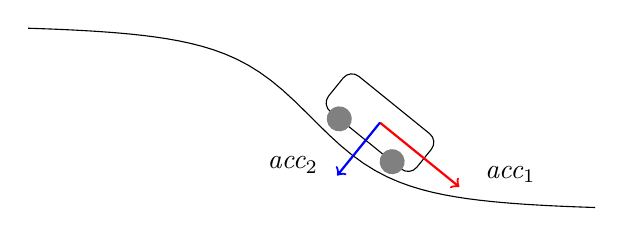
\begin{tikzpicture}[scale=1.2,samples=50,domain=-3:3]
\draw plot (\x,{(-\x/sqrt(\x*\x+1)});
\begin{scope}[xshift=3pt,yshift=4pt,scale=.6,rotate=-39]
\draw[rounded corners] (0,0) -- (0,.8) -- (2, .8) -- (2,0) -- cycle;
\draw[fill,gray] (.4,0) circle[radius=6pt];
\draw[fill,gray] (1.6,0) circle[radius=6pt];
\draw[->,red,thick] (1,.4) -- +(1.8,0);
\draw[->,blue,thick] (1,.4) -- +(0,-1.2);
\end{scope}
\node at (2.1,-.6) {$\textit{acc}_1$};
\node at (-.2,-.5) {$\textit{acc}_2$};
\end{tikzpicture}
\end{center}
\caption{Um robô com acelerômetros movendo-se em terreno difícil}\label{fig.slopes}
\end{figure}

A figura~\ref{fig.slopemes} mostra os dados adquiridos durante uma sessão de treinamento à medida que o robô desce uma encosta. Quando o operador da sessão de treinamento determina que o robô é estável (classe $C_1$), ela inicia uma medida indicada por um vermelho $\times$; quando ela determina que o robô está em uma situação perigosa (classe $C_2$), ela inicia uma medida indicada por um triângulo preto. O desafio é encontrar uma maneira de distinguir as amostras das duas classes.

\begin{figure}
\begin{center}
\includegraphics[width=\textwidth]{slope-allmu.pdf}
\end{center}
\caption{Detecção de um declive perigoso usando dados dos acelerômetros}\label{fig.slopemes}
\end{figure}

As linhas tracejadas na figura mostram os meios para os dois conjuntos de dados. É claro que elas não nos ajudam a classificar os dados devido à grande sobreposição entre os dois conjuntos de amostras. Além disso, o LDA não é apropriado porque não há similaridade nas distribuições: amostras quando o robô é estável aparecem em muitas partes da trama, enquanto amostras de situações perigosas estão concentradas em uma pequena área ao redor de sua média.

\subsection{Classificação com perceptrons}

Um \emph{perceptron} é um neurônio artificial com uma estrutura específica (Fig.~\ref{fig.perceptron}). Ele tem uma unidade de soma com entradas $\{x_1,\ldots,x_n\}$ e cada entrada $x_i$ é multiplicada por um fator $w_i$ antes da soma. Um input adicional $x_0$ tem o valor constante $1$ para definir um viés independente dos inputs. A saída do perceptron é obtida aplicando uma função $f$ ao resultado da adição.

\begin{figure}
\begin{center}
\begin{tikzpicture}%
[node distance=1.5cm and 2cm, nn/.style={circle,draw,minimum size=16pt}]
% Inputs
\node at (0,4) (i1) {};
\node at (0,3) (i2) {};
\node at (0,2) (i3) {};
\node at (0,0) (in) {};
\foreach \y in {.5,.75,1,1.25,1.5} \node at (0,\y) {$.$};
\foreach \i in {i1,i2,i3,in}
  \draw (\i) [yshift=-4pt,xshift=-1pt] arc[start angle=-90, end angle=90, radius=4pt] {};
% Neuron
\pic at (4,2) { nnnode={neuron} };
\% Output
\node (output) [node distance=1.5cm and 1cm,right=of neuron] {};
\draw[->] (neuron) -- (output) node {$y$};
% Arrows to neuron
\draw[->] (i1) node [xshift=-12pt] {$x_0=1$} -- node[fill=white] {$w_0$} (neuron);
\draw[->] (i2) node [xshift=-5pt] {$x_1$} -- node[fill=white] {$w_1$} (neuron);
\draw[->] (i3) node [xshift=-5pt] {$x_2$} -- node[fill=white] {$w_2$} (neuron);
\draw[->] (in) node [xshift=-5pt] {$x_n$} -- node[fill=white] {$w_n$} (neuron);
\end{tikzpicture}
\end{center}
\caption{Um perceptron}\label{fig.perceptron}
\end{figure}

Quando usado como classificador, as entradas para o perceptron são os valores retornados pelos sensores para que uma amostra seja classificada e a saída será um dos dois valores que indicam a classe para a qual a amostra é atribuída. Normalmente, a função de saída $f$ é apenas o sinal da soma ponderada:
\begin{equation}
y=sign\left(\,\sum_{i=0}^{n} w_i\,x_i\,\right)=\pm 1\,,\label{eq.perceptron-output}
\end{equation}
onde uma classe corresponde a $+1$ e a outra a $-1$.

Os dados são normalizados para que todas as entradas estejam na mesma faixa, geralmente $-1\leq x_i\leq +1$. Os dados na Fig.~\ref{fig.slopemes} podem ser normalizados dividindo cada valor por $30$.

Dado um conjunto de valores de entrada $\{x_0=1,x_1,\ldots,x_n\}$ de uma amostra, o objetivo de uma sessão de treinamento é encontrar um conjunto de pesos $\{w_0,w_1,\ldots,w_n\}$ para que a saída seja o valor $\pm 1$ que atribui a amostra à classe correta.

Se a amostra estiver perto da borda entre duas classes, a soma ponderada será próxima a zero. Portanto, um perceptron é também um classificador linear: para distinguir entre saídas de $\pm 1$, o discriminante que divide as duas classes é definido pelo conjunto de pesos que dá uma saída de zero:
\[
\sum_{i=0}^{n} w_i\,x_i=0\,,
\]
ou
\begin{equation}
w_0 + w_1x_1 + \cdots + w_nx_n = 0\,.\label{eq.perceptron-disc}
\end{equation}
A apresentação do LDA para um problema bidimensional ($n=2$) levou ao Eq.~\ref{eq.diseq}, que é o mesmo que Eq.~\ref{eq.perceptron-disc} quando $c=-w_0$. A diferença entre as duas abordagens está na forma como os pesos são obtidos: em LDA as estatísticas são usadas enquanto para perceptrons elas resultam de um processo de aprendizado iterativo.

\subsection{Aprendendo por um perceptron}

A busca iterativa dos valores dos pesos $\{w_0,w_1,\ldots,w_n\}$ começa definindo-os para um valor pequeno, como $0,1$. Durante a fase de aprendizagem, um conjunto de amostras é apresentado ao perceptron, juntamente com o resultado esperado (a classe) para cada elemento do conjunto. O conjunto de amostras deve ser construído de forma aleatória e incluir elementos de todas as classes; além disso, os elementos de uma única classe também devem ser escolhidos aleatoriamente. Isto é para evitar que o algoritmo de aprendizado gere uma discriminação que seja ótima em uma situação específica, e para assegurar que o processo converge rapidamente para uma discriminação geral ótima, ao invés de gastar muito tempo otimizando para casos específicos.

O ajuste dos pesos é calculado da seguinte forma:
\begin{equation}
w_i(t+1) = w_i(t) + \eta \,x_i \,y\,,\;\;0\leq i \leq n\,.\label{eq.perceptron-learn}
\end{equation}
Esta é essencialmente a regra Hebbiana para as ANNs (Eq.~\ref{eq.hebbian}). $w_i(t)$ e $w_i(t+1)$ são os pesos $i$'th antes e depois da correção, $\eta$ define a taxa de aprendizagem, $x_i$ é a entrada normalizada, e $y$ é a saída desejada. Como a função de sinal é aplicada à soma das entradas ponderadas, $y$ é $1$ ou $-1$, exceto nas raras ocasiões em que a soma é exatamente zero. 

O Eq.~\ref{eq.perceptron-learn} corrige os pesos adicionando ou subtraindo um valor que é proporcional à entrada, onde o coeficiente de proporcionalidade é a taxa de aprendizado. Um valor pequeno para a taxa de aprendizado significa que as correções dos pesos serão em pequenos incrementos, enquanto uma alta taxa de aprendizado fará com que as correções dos pesos sejam em incrementos maiores. Uma vez concluído o aprendizado, os pesos são usados para classificar as amostras subseqüentes.

Algoritmos~\ref{alg.perceptron1}--\ref{alg.perceptron2} são uma descrição formal da classificação por perceptrons. A constante $N$ é o tamanho do conjunto de amostras para a fase de aprendizagem, enquanto $n$ é o número de valores dos sensores retornados para cada amostra.

\begin{figure}
\begin{alg}{Classificação por um perceptron (fase de aprendizagem)}{perceptron1}
\hline
&\idv{}float array[$N$,$n$] $\vec{X}$&// Set of samples\\
&\idv{}float array[$n+1$] $\vec{w}$ \ass{} $[0.1,0.1,\ldots]$&// Weights\\
&\idv{}float array[$n$] $\vec{x}$&// Random sample\\
&\idv{}integer $c$&// Class of the random sample\\
&\idv{}integer $y$&// Output of the perceptron\\
\hline
\stl{}&loop until learning terminated&\\ 
\stl{}&\idc{}$\vec{x}$ \ass random element of $\vec{X}$&\\
\stl{}&\idc{}$c$ \ass class to which $\vec{x}$ belongs&\\
\stl{}&\idc{}$y$ \ass output according to Eq.~\ref{eq.perceptron-output}&\\
\stl{}&\idc{}if $y$ does not correspond to class $c$&\\
\stl{}&\idc{}\idc{}adjust $w_i$ according to Eq.~\ref{eq.perceptron-learn}&\\
\stl{}&Output $\vec{w}$&\\
\end{alg}
\end{figure}

\begin{figure}
\begin{alg}{Classificação por um perceptron (fase de reconhecimento)}{perceptron2}
&\idv{}float $\vec{w}$ \ass weights from the learning phase&\\
&\idv{}float $\vec{x}$&\\
&\idv{}integer $y$&\\
\hline
\stl{}&loop&\\
\stl{}&\idc{}$\vec{x}$ \ass new sample&\\
\stl{}&\idc{}$y$ \ass output of perceptron for $\vec{x},\vec{w}$&\\
\stl{}&\idc{}if $y=1$&\\
\stl{}&\idc{}\idc{}assign $\vec{x}$ to class $C_1$&\\
\stl{}&\idc{}else if $y=-1$&\\
\stl{}&\idc{}\idc{}assign $\vec{x}$ to class $C_2$&\\
\end{alg}
\end{figure}

Quando a fase de aprendizagem deve ser encerrada? Pode-se especificar um valor arbitrário, por exemplo: encerrar a fase de aprendizagem quando $98\%$ das amostras forem classificadas corretamente. Entretanto, pode não ser possível atingir este nível. Um método melhor é encerrar a fase de aprendizagem quando a magnitude das correções dos pesos se torna pequena.

\subsection{Exemplo numérico}

Voltamos ao robô que está aprendendo a evitar inclinações perigosas e aplicamos o algoritmo de aprendizagem aos dados da Fig.~\ref{fig.slopemes}. O perceptron tem três entradas: $x_0$, que sempre é de $1$, $x_1$ para os dados do acelerômetro frontal/traseiro, e $x_2$ para os dados do acelerômetro para cima/para baixo. Os dados são normalizados dividindo cada amostra por $30$ para que os valores fiquem entre $0$ e $1$. Especificamos que uma saída de $1$ corresponde à classe $C_1$ (estável) e uma saída de $-1$ corresponde à classe $C_2$ (perigosa).

Selecione uma amostra aleatória dos dados de entrada, por exemplo, uma amostra na classe $C_1$ cujos valores de sensor são $x_{1}=14$ e $x_{2}=18$. A entrada normalizada é $x_{1}=14/30=0,47$ e $x_{2}=18/30=0,6$. A saída do perceptron com pesos iniciais $0,1$ é:
\begin{eqnarray*}
y &=& \mathit{sign}(w_0\times 1 + w_1x_1 + w_2x_2)\\
&=& \mathit{sign}(0.1\times 1 + 0.1\times 0.47 + 0.1\times 0.6)\\
&=& \mathit{sign}(0.207)\\
&=& 1\,.
\end{eqnarray*}
Esta saída é correta, portanto, os pesos não precisam ser corrigidos. Agora escolha uma amostra aleatória na classe $C_2$ cujos valores do sensor sejam $x_{1}=17$ e $x_{2}=15$. A entrada normalizada é $x_{1}=17/30=0,57$ e $x_{2}=15/30=0,5$. A saída do perceptron é:
\begin{eqnarray*}
y &=& \mathit{sign}(w_0\times 1 + w_1x_1 + w_2x_2)\\
&=& \mathit{sign}(0.1\times 1 + 0.1\times 0.57 + 0.1\times 0.5)\\
&=& \mathit{sign}(0.207)\\
&=& 1\,.
\end{eqnarray*}
Esta saída não é correta: a amostra é da classe $C_2$ que corresponde a $-1$. Os pesos são agora ajustados usando Eq.~\ref{eq.perceptron-learn} com uma taxa de aprendizagem $\eta = 0,1$:
\[
\spacearray
\begin{array}{lclclcl}
w_0(t+1) &=& w_0(t) + \eta \,x_0 y &=& 0.1 + 0.1\times 1\times -1 &=& 0 \\
w_1(t+1) &=& w_1(t) + \eta \,x_1 y &=& 0.1 + 0.1\times 0.57\times-1 &=& 0.043 \\
w_2(t+1) &=& w_2(t) + \eta \,x_2 y &=& 0.1 + 0.1\times 0.5\times -1 &=& 0.05\,.
\end{array}
\]
Estes serão os novos pesos para a próxima iteração. Se continuarmos por $2000$ iterações, os pesos evoluem como mostrado na Fig.~\ref{fig.weights-fixeta}. No final do processo de aprendizagem, os pesos estão:
\[
w_0 = -0.1,\;\;\; w_1 = -0.39,\;\;\; w_2 = 0.53\,.
\]

\begin{figure}[bt]
\begin{center}
\includegraphics[width=0.8\textwidth]{weights.pdf}
\end{center}
\caption{Evolução dos pesos para a aprendizagem por um perceptron}\label{fig.weights-fixeta}
\end{figure}

Estes pesos podem agora ser utilizados na fase de reconhecimento da classificação Algoritmo~\ref{alg.perceptron2}. A linha discriminante construída pelo perceptron (Eq.~\ref{eq.perceptron-disc}) é:
\[
-0.1 -0.39x_1 + 0.53x_2 = 0\,.
\]
As coordenadas desta linha são os valores normalizados, mas eles podem ser transformados novamente nos valores brutos obtidos dos acelerômetros. A linha é mostrada na Fig.~\ref{fig.perceptron-dis} e considerando a grande sobreposição das classes, ela faz um trabalho razoavelmente bom de distinção entre elas.

\begin{figure}
\begin{center}
\includegraphics[width=0.9\textwidth]{perceptron-discrim.pdf}
\end{center}
\caption{Linha discriminante computada a partir dos pesos de perceptron}\label{fig.perceptron-dis}
\end{figure}

\subsection{Afinação dos parâmetros do perceptron}

O desempenho de um perceptron é determinado pelo número de iterações e pela taxa de aprendizagem. A figura~\ref{fig.weights-fixeta} mostra que há uma forte variação nos pesos no início, mas os pesos se estabilizam à medida que o número de iterações aumenta. Assim, é relativamente simples monitorar os pesos e encerrar o cálculo quando os pesos se estabilizam.

Esta evolução dos pesos depende fortemente da taxa de aprendizado. Aumentar a taxa de aprendizado acelera a variação no início, mas correções fortes não são benéficas quando os pesos começam a se estabilizar. A partir da Fig.~\ref{fig.weights-fixeta}, fica claro que, mesmo no final da corrida, há variações significativas nos pesos que oscilam em torno do valor ótimo. Isto sugere que reduzimos a taxa de aprendizagem para reduzir as oscilações, mas isso irá retardar a convergência para os pesos ótimos no início da fase de aprendizagem.

A solução é usar uma taxa de aprendizagem variável que não seja constante. Ela deve começar grande para incentivar a convergência rápida para os valores ótimos, e depois se tornar menor para reduzir as oscilações. Por exemplo, podemos começar com a taxa de aprendizagem de $0,1$ e depois reduzi-la continuamente usando a equação:
\[
\eta\,(t+1) = \eta\,(t) \times 0.997\,.
\]
A figura~\ref{fig.perceptron-dis-etavar} mostra a evolução dos pesos quando esta taxa de aprendizagem variável é utilizada. A diminuição exponencial de $\eta$ também é plotada na figura. Uma comparação entre Fig.~\ref{fig.weights-fixeta} e Fig.~\ref{fig.perceptron-dis-etavar} mostra claramente a superioridade da taxa de aprendizagem variável e esta melhoria é obtida com muito pouco cálculo adicional.
\begin{figure}
\begin{center}
\includegraphics[width=0.9\textwidth]{weights-etavar.pdf}
\end{center}
\caption{Evolução dos pesos para aprendizagem por um perceptron com uma taxa de aprendizagem variável}\label{fig.perceptron-dis-etavar}
\end{figure}

\begin{framed}
\act{Aprendendo com um perceptron}{perceptronlearn}
\begin{itemize}
\item Faça um conjunto de medidas dos acelerômetros em seu robô em várias inclinações e trace os dados. Para cada amostra, você terá que decidir se o robô corre o risco de cair da encosta.
\item Classificar os dados usando um perceptron. Que linha discriminante você encontra?
\item Use um perceptron para classificar as áreas cinzentas usando os dados da Activity~\ref{act.LDAchameleon}. Que discriminante você acha? Compare o discriminante encontrado pelo perceptron com o discriminante encontrado pela LDA.
\end{itemize}
\end{framed}

\section{Sumário}

Amostras de duas classes podem ser distinguidas usando apenas seus meios ou usando tanto os meios como as variâncias. A análise linear discriminante é um método de classificação que se baseia no cálculo das covariâncias entre as amostras das classes. A LDA só tem um bom desempenho quando as distribuições das amostras das classes são semelhantes. Quando esta suposição não se mantém, perceptrons podem ser usados. Para um ótimo desempenho, a taxa de aprendizagem de um perceptron deve ser ajustada, se possível dinamicamente durante a fase de aprendizagem.

\section{Leitura adicional}

Uma apresentação matemática detalhada da análise linear discriminante pode ser encontrada em Izenman~\cite[Chapter~8]{izenman2008}. Os livros didáticos sobre técnicas de aprendizagem de máquinas são \cite{harrington2012machine, kubat2015machinelearning}.
